% (c) 2020 Stefan Antonowicz
% Based off of tex found at https://github.com/ludus-leonis/nipajin
% This file is released under Creative Commons Attribution-NonCommercial-ShareAlike 4.0 International License.
% Please do not apply other licenses one-way.

\mysection{The Spheres}{the-spheres}

\flavor {
I have seen the dark universe yawning

Where the black planets roll without aim,

Where they roll in their horror unheeded,

Without knowledge, or lustre, or name. 

\Tilde H.P. Lovecraft, \myital{Nemesis}

}

    The Totality is everything, and everything is the Totality. At the heart of the Totality lies the Void, and at the center of the Void grows the Tree of Ygg, and on one of the unending shoots on one of the eternal branches inside one of the trillion trillion plumules blooms a flower - the Dream. Inside the Dream \TheAuthority dreams reality, and in one dreamed universe, at an off-center point of a lenticular galaxy, there is a planet.

    This planet - a purple gas giant - spins slowly around a star in a modest elliptical orbit; around this Goliath five equidistant moons whirl in a gravitational dance.  Mortals name him \mybold{Tartarus}, the star around which he orbits \mybold{Helios}, and the moons they dwell upon the \mybold{Five Dwarfs}:  \mybold{Acheron, Cocytus, Phlegethon, Styx, and Lethe}.

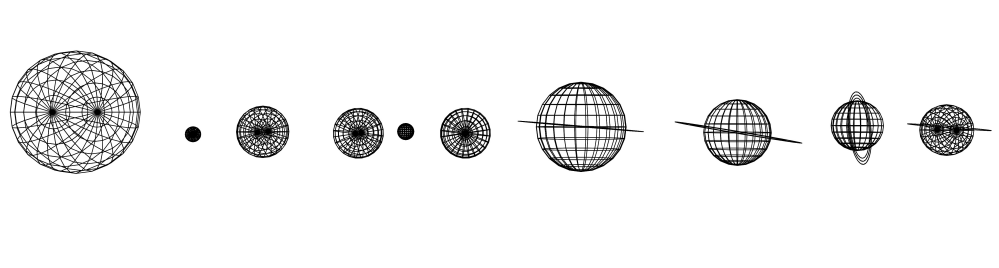
\includegraphics[width=\linewidth,keepaspectratio=true]{totality/SpheresHeader}

    From any moon you can see two of its brothers; in the morning light from Helios, Tartarus looms faintly on the horizon. As the day progresses the Scythe appears, Helios illuminating a crescent of the visible side of the purple giant, the signal for him to begin waxing to fullness and heralding the coming of night. At dusk Helios provides light like candlelight, the shadows lengthening as the night progresses, until Tartarus hides his face. The moons of Tartarus glow brightly, but it is darkest before dawn, as Helios rises and behind Tartarus in a spectacular daily eclipse that throws the world into pitch darkness. It is a time of great mischief, fear, and terror - until Helios peeks her face from behind Tartarus to begin the wheel anew.


